\begin{lstlisting}
•    Section 4.1: 2, 6, 8  
•    Section 4.2: 3, 9, 10
\end{lstlisting}
\begin{figure}[H]
\centering
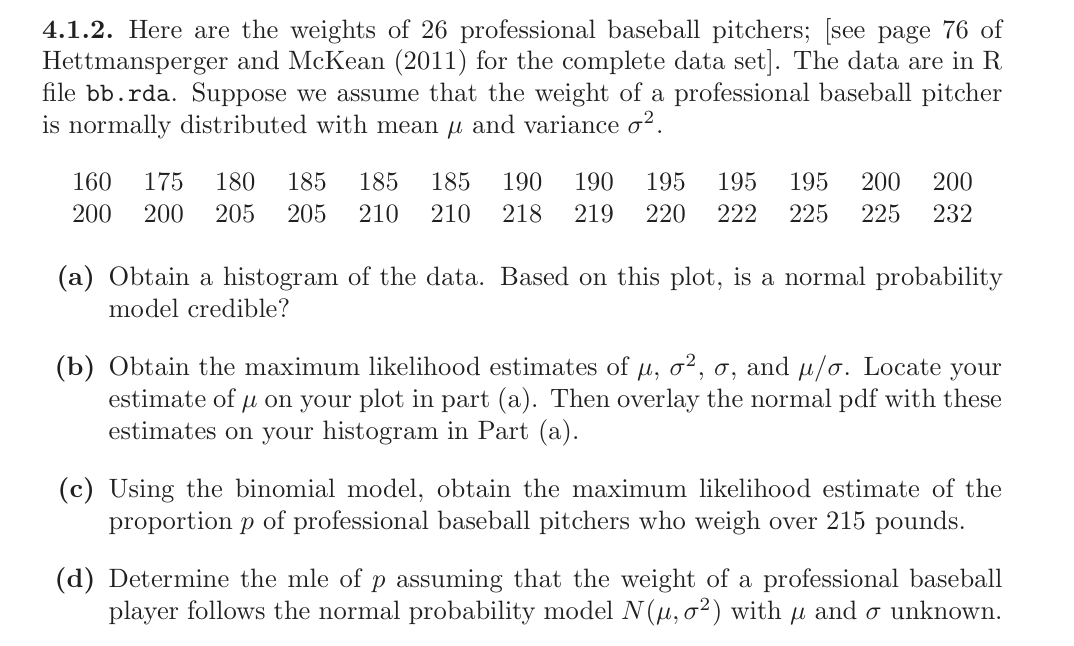
\includegraphics[width=\textwidth]{hw4-20250321.png}
% \caption{}
\label{}
\end{figure}

(a)
\begin{figure}[H]
\centering
\includegraphics[width=\textwidth]{Figure_1.png}
% \caption{}
\label{}
\end{figure}
The normal probability model is credible.

(b)
For normal distributions, the mles are
\[
\widehat{\mu}=\overline{X}=201
\]
\[
\widehat{\sigma }^{2}=n^{-1}\sum_{i=1}^{n} (X_i-\overline{X})^{2}=293.923
\]
\[
\widehat{\sigma}=\sqrt{ 293.923 }\approx17.145
\]
\[
\widehat{(\mu/\sigma)}=\widehat{\mu}/\widehat{\sigma}\approx11.723
\]
Locate $\widehat{\mu}$ on the plot:
\begin{figure}[H]
\centering
\includegraphics[width=\textwidth]{Figure_1 1.png}
% \caption{}
\label{}
\end{figure}

Overlay the normal pdf with these estimates:
\begin{figure}[H]
\centering
\includegraphics[width=\textwidth]{Figure_1 2.png}
% \caption{}
\label{}
\end{figure}

(c)
\[
L(p)={\binom{n}{X} }p^{X}(1-p)^{n-X}
\]
where $X$ is the number of successes (pitchers weighing over 215 pounds) and $p$ is the probability of success (a pitcher weighing over 215 pounds).
\[
\begin{aligned}
\frac{dL(p)}{dp} & ={\binom{n}{X} }(Xp^{X-1}(1-p)^{n-X}-p^{X}(n-X)(1-p)^{n-X-1}) \\
 & ={\binom{n}{X} }p^{X-1}(1-p)^{n-X-1}(X(1-p)-(n-X)p) \\
 & ={\binom{n}{X} }p^{X-1}(1-p)^{n-X-1}(X-np)
\end{aligned}
\]
Let $\frac{dL(p)}{dp}=0$ then
\[
\widehat{p}=\frac{X}{n}=\frac{7}{26}
\]
(d)
\[
p=P(X>215)=1-\Phi\left( \frac{215-\mu}{\sigma} \right)
\]
where $\Phi$ is the CDF of the standard normal distribution $N(0,1)$. Then
\[
\widehat{p}=1-\Phi\left( \frac{215-\widehat{\mu}}{\widehat{\sigma}} \right)\approx0.207
\]
\begin{figure}[H]
\centering
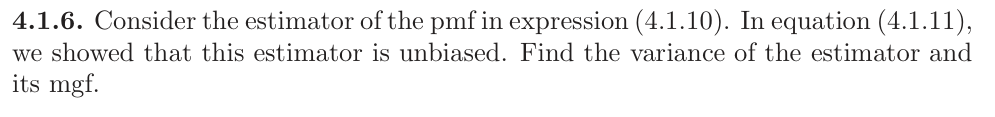
\includegraphics[width=\textwidth]{1-hw4-20250321.png}
% \caption{}
\label{}
\end{figure}

The estimator
\[
\widehat{p}(a_j)=\frac{1}{n}\sum_{i=1}^{n} I_j(X_i)
\]
where
\[
I_j(X_i)=\begin{cases}
1 & X_i=a_j \\
0 & X_i\neq a_j.
\end{cases}
\]
Its variance is
\[
\begin{aligned}
\mathrm{Var}(\widehat{p}(a_j)) & =E[\widehat{p}(a_j)^{2}]-(E[\widehat{p}(a_j)])^{2} \\
 & =E\left[ \left( \frac{1}{n}\sum_{i=1}^{n} I_j(X_i) \right)^{2} \right]-p(a_j)^{2} \\
 & =\frac{1}{n^{2}}\sum_{i,k=1}^{n} E[I_j(X_i)I_j(X_k)]-p(a_j)^{2} \\
 & =\frac{2}{n^{2}}\sum_{1\leq i<k\leq n}\underbrace{ E[I_j(X_i)I_j(X_k)] }_{ =E[I_j(X_i)]E[I_j(X_k)] }+\frac{1}{n^{2}}\cdot n\sum_{i=1}^{n} E[I^{2}_j(X_i)]-p(a_j)^{2} \\
 & =\frac{1}{n^{2}}n(n-1) p(a_j)^{2}+\frac{1}{n}p(a_j)-p(a_j)^{2} \\
 & =\frac{1}{n}(p(a_j)-p(a_j)^{2})
\end{aligned}
\]
Its mgf is
\[
\begin{aligned}
M(t) & =E[e^{ \widehat{p}(a_j)t }]=E\left[ \exp \left\{  \frac{1}{n}\sum_{i=1}^{n} I_j(X_i)t  \right\} \right] \\
 & =\prod_{i=1}^{n} E\left[ \exp \left\{  I_j(X_i)\frac{t}{n}  \right\} \right]   \\
 & =\prod_{i=1}^{n} \left( 1-p(a_j)+p(a_j)e^{ \frac{t}{n} } \right) \\
 & =(1+p(a_j)(e^{ \frac{t}{n} }-1))^{n}
\end{aligned}
\]
\begin{figure}[H]
\centering
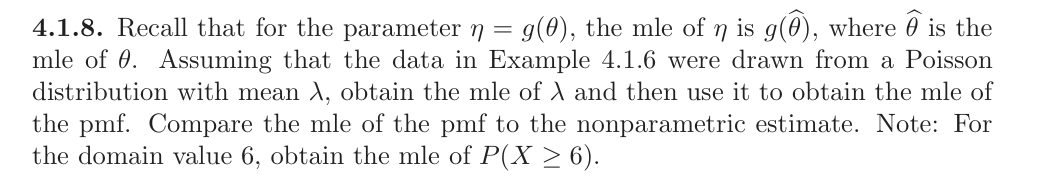
\includegraphics[width=\textwidth]{2-hw4-20250321.png}
% \caption{}
\label{}
\end{figure}

For Poisson distribution with mean $\lambda$, we have
\[
P(X=k)=\frac{\lambda^{k}e^{ -\lambda }}{k!},\qquad k=0,1,2,\dots
\]
The likelihood function is
\[
l(\lambda)=\sum_{i=1}^{n} \log\frac{\lambda^{x_i}e^{ -\lambda }}{x_i!}=-n\lambda+(\log\lambda)\cdot \sum_{i=1}^{n} x_i-\sum_{i=1}^{n} \log (x_i!)
\]
The first parital of the log-likelihood with respect to $\lambda$ is
\[
\frac{ \partial l(\lambda) }{ \partial \lambda } =-n+\frac{1}{\lambda}\sum_{i=1}^{n} x_i
\]
Setting this partial to 0 and solving for $\lambda$, we obtain the solution $\frac{1}{n}\sum_{i=1}^{n}x_i$, thus the mle of $\lambda$ is
\[
\widehat{\lambda}=\frac{1}{n}\sum_{i=1}^{n} X_i=\overline{X}=\frac{64}{30}\approx2.133
\]
The mle of the pmf is
\[
P(X=j)=\frac{\widehat{\lambda}^{j}e^{ -\widehat{\lambda} }}{j!}=\frac{\left( \frac{32}{15}  \right)^{j}e^{ -\frac{32}{15}  }}{j!},\qquad j=0,1,2,\dots
\]
\[
P(X\geq 6)=0.0218705
\]
\begin{figure}[H]
\centering
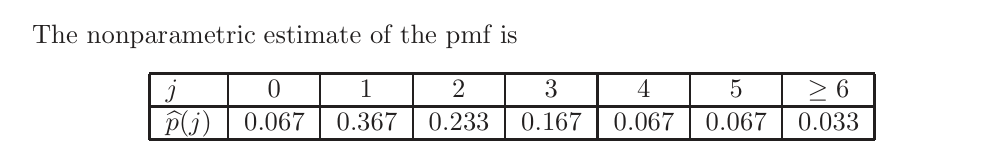
\includegraphics[width=\textwidth]{6-hw4-20250321.png}
% \caption{}
\label{}
\end{figure}

\begin{table}[h]
	\centering
	\begin{tabular}{|c|c|c|c|c|c|c|c|}
		\hline
		$j$ & 0 & 1 & 2 & 3 & 4 & 5 & $\geq6$ \\
		\hline
		$p(j)$ & 0.118442 & 0.252676 & 0.269521 & 0.191659 & 0.102218 & 0.0436132 & 0.0218705 \\
		\hline
	\end{tabular}
\end{table}
\begin{figure}[H]
\centering
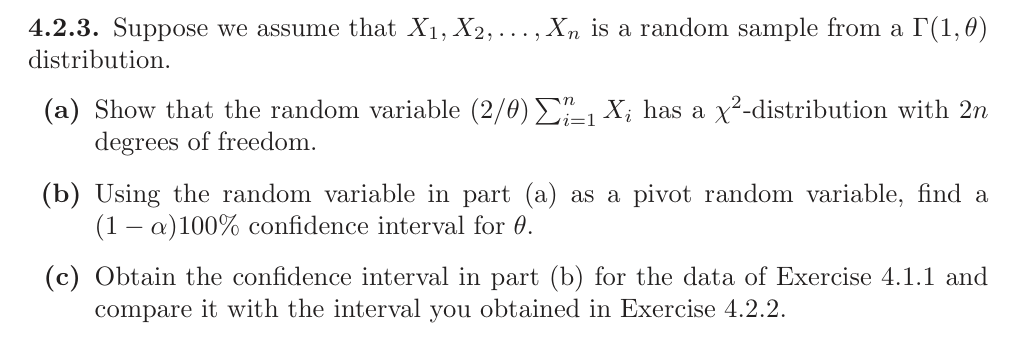
\includegraphics[width=\textwidth]{3-hw4-20250321.png}
% \caption{}
\label{}
\end{figure}

\begin{proof}
(a) The characteristic function of $X_j$ is
\[
\varphi_{X_j}(t)=\left( 1-it\theta \right)^{-1}
\]
Then the characteristic function of $Y=(2/\theta)\sum_{i=1}^{n}X_i$ is
\[
\varphi_{Y}(t)=\prod_{j=1}^{n} \varphi_{X_j}(2t/\theta)=\prod_{j=1}^{n} \left( 1-2it \right)^{-1}=(1-2it)^{-n}
\]
Then $Y\sim \chi^{2}(2n)$.

(b) define $t_{\alpha,2n}$ to be the upper $\alpha/2$ critical point of a $\chi^{2}$ -distribution with $2n$ degrees of freedom, i.e. $\alpha =P(Y>t_{\alpha,2n})$. Using a simple algebraic derivation, we obtain
\[
\begin{aligned}
1-\alpha & =P(Y<t_{\alpha,2n}) \\
 &  =P_{\theta}\left( \frac{2}{\theta} \sum_{i=1}^{n} X_i<t_{\alpha,2n} \right) \\
 & =P_{\theta}\left( \frac{2n\overline{X}}{\theta}<t_{\alpha,2n} \right) \\
 & =P_{\theta}\left( \theta>\frac{2n\overline{X}}{t_{\alpha,2n}} \right)
\end{aligned}
\]
Then  an approximate $(1-\alpha) 100\%$ confidence interval for $\theta$ is given by
\[
\left( \frac{2n\overline{x}}{t_{\alpha,2n}},+\infty \right)
\]
(c)

\begin{figure}[H]
\centering
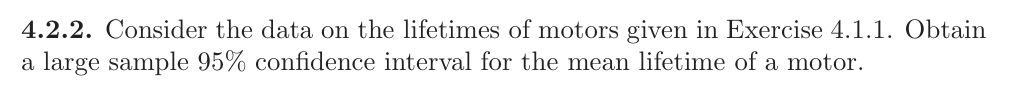
\includegraphics[width=\textwidth]{hw4-20250322.png}
% \caption{}
\label{}
\end{figure}

\begin{figure}[H]
\centering
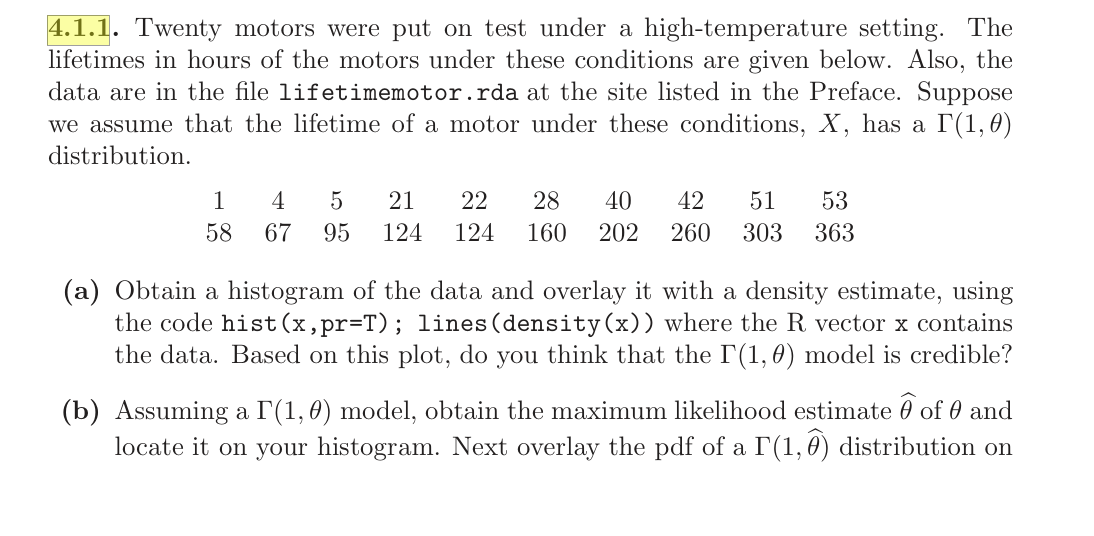
\includegraphics[width=\textwidth]{1-hw4-20250322.png}
% \caption{}
\label{}
\end{figure}

\end{proof}

\begin{figure}[H]
\centering
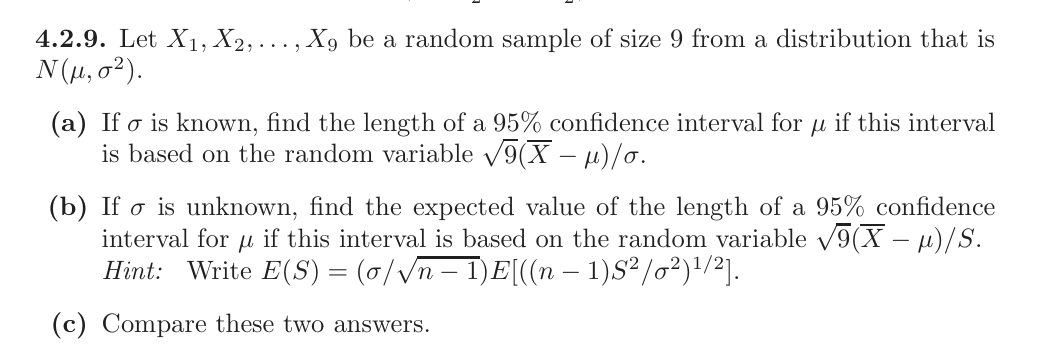
\includegraphics[width=\textwidth]{4-hw4-20250321.png}
% \caption{}
\label{}
\end{figure}

(a)
\[
\overline{X}\sim N(\mu,\sigma^{2}/9)
\]
$\alpha=0.05$, and $z_{\frac{\alpha}{2}}$ means $\frac{\alpha}{2}=P\left( Y>z_{\frac{\alpha}{2}} \right)$, where $Y=\frac{\sqrt{ 9 }(\overline{X}-\mu)}{\sigma}\sim N(0,1)$. We obtain
\[
\begin{aligned}
1-\alpha & =P\left( -z_{\frac{\alpha}{2}}<Y <z_{\frac{\alpha}{2}}\right) \\
 & =P_{\mu}\left( -z_{\frac{\alpha}{2}}<\frac{\sqrt{ 9 }(\overline{X}-\mu)}{\sigma}<z_{\frac{\alpha}{2}} \right) \\
 & =P_{\mu}\left( \overline{X}-z_{\frac{\alpha}{2}}\cdot\frac{\sigma}{3}<\mu<\overline{X}+z_{\frac{\alpha}{2}}\cdot\frac{\sigma}{3} \right)
\end{aligned}
\]
Then a $95\%$ confidence interval for $\mu$ is given by
\[
\left( \overline{x}-z_{\frac{\alpha}{2}}\cdot\frac{\sigma}{3},\overline{x}+z_{\frac{\alpha}{2}}\cdot\frac{\sigma}{3} \right)
\]
(b)
By student's theorem, the rv $T=(\overline{X}-\mu)/(S/\sqrt{ 9 })$ has a $t$ -distribution with $9-1=8$ degrees of freedom. Define
\[
\frac{\alpha}{2}=P(T>t_{\alpha/2,8})
\]
We obtain
\[
\begin{aligned}
1-\alpha & =P(-t_{\alpha/2,8}<T<t_{\alpha/2,8} ) \\
 & =P_{\mu}\left( -t_{\alpha/2,8}<\frac{\overline{X}-\mu}{S/\sqrt{ 9 }} \right)<t_{\alpha/2,8}  \\
 & =P_{\mu}\left( \overline{X}-t_{\alpha /2,8}\cdot \frac{S}{3}<\mu<\overline{X}+t_{\alpha/2,8}\cdot \frac{S}{3} \right)
\end{aligned}
\]
Then a $95\%$ confidence interval for $\mu$ is given by
\[
\left( \overline{x}-t_{\alpha/2,8}\cdot \frac{S}{3},\overline{x}+t_{\alpha/2,8}\cdot \frac{S}{3} \right)
\]
(c)
Omitted

\begin{figure}[H]
\centering
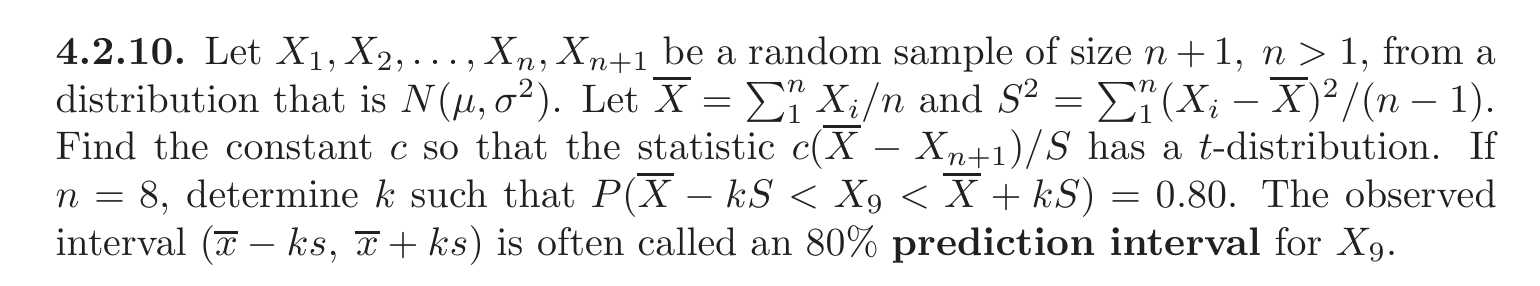
\includegraphics[width=\textwidth]{5-hw4-20250321.png}
% \caption{}
\label{}
\end{figure}
\[
(n-1)S^{2}/\sigma^{2}\sim \chi^{2}(n-1)
\]
\[
\overline{X}\sim N(\mu,\sigma^{2}/n)
\]
Then
\[
\overline{X}-X_{n+1}\sim N\left( 0,\frac{n+1}{n}\sigma^{2} \right)
\]
Then
\[
\sqrt{ \frac{n}{n+1} }\cdot\frac{1}{\sigma}\cdot (\overline{X}-X_{n+1})\sim N(0,1)
\]
By the defintion of $t$ -distribution, the rv
\[
T=\frac{\sqrt{ n/(n+1) }\cdot\frac{1}{\sigma}\cdot (\overline{X}-X_{n+1})}{\sqrt{ \frac{(n-1)S^{2}/\sigma^{2}}{n-1} }}=\sqrt{ \frac{n}{n+1}  }\cdot\frac{\overline{X}-X_{n+1}}{S}
\]
has a $t$ -distribution with $r=n-1$. Thus
\[
c=\sqrt{ \frac{n}{n+1}  }
\]
Denote $t_{\alpha/2,n-1}$ to be $\frac{\alpha}{2}=P(T>t_{\alpha/2,n-1})$. Then
\[
\begin{aligned}
1-\alpha & =P(-t_{\alpha/2,n-1}<T<t_{\alpha/2,n-1} )  \\
 & =P\left( -t_{\alpha/2,n-1}<\sqrt{ \frac{n}{n+1}  }\cdot\frac{\overline{X}-X_{n+1}}{S}<t_{\alpha/2,n-1} \right) \\
 & =P\left( \overline{X}-\sqrt{ \frac{n+1}{n} }S\cdot t_{\alpha/2,n-1}<X_{n+1}< \overline{X}+\sqrt{ \frac{n+1}{n} }S\cdot t_{\alpha/2,n-1} \right) \\
\end{aligned}
\]
Then the $(1-\alpha) 100\%$ confidence interval for $X_{n+1}$ is given by
\[
\left( \overline{x}-\sqrt{ \frac{n+1}{n} }s\cdot t_{\alpha/2,n-1} ,\overline{x}+\sqrt{ \frac{n+1}{n} }s\cdot t_{\alpha/2,n-1}\right)
\]
Then
\[
k=\frac{3}{2\sqrt{ 2 }}\cdot t_{0.1,7}\approx\frac{3}{2\sqrt{ 2 }}\cdot1.415\approx1.5
\]